\documentclass[11pt]{scrartcl} % Font size

%%%%%%%%%%%%%%%%%%%%%%%%%%%%%%%%%%%%%%%%%
% Wenneker Assignment
% Structure Specification File
% Version 2.0 (12/1/2019)
%
% This template originates from:
% http://www.LaTeXTemplates.com
%
% Authors:
% Vel (vel@LaTeXTemplates.com)
% Frits Wenneker
%
% License:
% CC BY-NC-SA 3.0 (http://creativecommons.org/licenses/by-nc-sa/3.0/)
%
%%%%%%%%%%%%%%%%%%%%%%%%%%%%%%%%%%%%%%%%%

%----------------------------------------------------------------------------------------
%	PACKAGES AND OTHER DOCUMENT CONFIGURATIONS
%----------------------------------------------------------------------------------------

\usepackage{amsmath, amsfonts, amsthm} % Math packages

\usepackage{listings} % Code listings, with syntax highlighting

\usepackage[english]{babel} % English language hyphenation

\usepackage[xetex]{graphicx}
%\usepackage{graphicx} % Required for inserting images
\graphicspath{{Figures/}{./}} % Specifies where to look for included images (trailing slash required)

\usepackage{booktabs} % Required for better horizontal rules in tables

\numberwithin{equation}{section} % Number equations within sections (i.e. 1.1, 1.2, 2.1, 2.2 instead of 1, 2, 3, 4)
\numberwithin{figure}{section} % Number figures within sections (i.e. 1.1, 1.2, 2.1, 2.2 instead of 1, 2, 3, 4)
\numberwithin{table}{section} % Number tables within sections (i.e. 1.1, 1.2, 2.1, 2.2 instead of 1, 2, 3, 4)

\setlength\parindent{0pt} % Removes all indentation from paragraphs

\usepackage{enumitem} % Required for list customisation
\setlist{noitemsep} % No spacing between list items

%----------------------------------------------------------------------------------------
%	DOCUMENT MARGINS
%----------------------------------------------------------------------------------------

\usepackage{geometry} % Required for adjusting page dimensions and margins

\geometry{
	paper=a4paper, % Paper size, change to letterpaper for US letter size
	top=2.5cm, % Top margin
	bottom=3cm, % Bottom margin
	left=3cm, % Left margin
	right=3cm, % Right margin
	headheight=0.75cm, % Header height
	footskip=1.5cm, % Space from the bottom margin to the baseline of the footer
	headsep=0.75cm, % Space from the top margin to the baseline of the header
	%showframe, % Uncomment to show how the type block is set on the page
}

%----------------------------------------------------------------------------------------
%	FONTS
%----------------------------------------------------------------------------------------

\usepackage[utf8]{inputenc} % Required for inputting international characters
\usepackage[T1]{fontenc} % Use 8-bit encoding

\usepackage{fourier} % Use the Adobe Utopia font for the document

%----------------------------------------------------------------------------------------
%	SECTION TITLES
%----------------------------------------------------------------------------------------

\usepackage{sectsty} % Allows customising section commands

\sectionfont{\vspace{6pt}\centering\normalfont\scshape} % \section{} styling
\subsectionfont{\normalfont\bfseries} % \subsection{} styling
\subsubsectionfont{\normalfont\itshape} % \subsubsection{} styling
\paragraphfont{\normalfont\scshape} % \paragraph{} styling

%----------------------------------------------------------------------------------------
%	HEADERS AND FOOTERS
%----------------------------------------------------------------------------------------

\usepackage{scrlayer-scrpage} % Required for customising headers and footers

\ohead*{} % Right header
\ihead*{} % Left header
\chead*{} % Centre header

\ofoot*{} % Right footer
\ifoot*{} % Left footer
\cfoot*{\pagemark} % Centre footer
 % Include the file specifying the document structure and custom commands
% LaTeX settings for MATLAB code listings
% based on Ted Pavlic's settings in http://links.tedpavlic.com/ascii/homework_new_tex.ascii
\usepackage{listings}
\usepackage[usenames,dvipsnames]{color}

% This is the color used for MATLAB comments below
\definecolor{MyDarkGreen}{rgb}{0.0,0.4,0.0}

% For faster processing, load Matlab syntax for listings
\lstloadlanguages{Matlab}%
\lstset{language=Matlab,                        % Use MATLAB
        frame=single,                           % Single frame around code
        basicstyle=\scriptsize\ttfamily,             % Use small true type font
        keywordstyle=[1]\color{Blue}\bfseries,        % MATLAB functions bold and blue
        keywordstyle=[2]\color{Purple},         % MATLAB function arguments purple
        keywordstyle=[3]\color{Blue}\underbar,  % User functions underlined and blue
        identifierstyle=,                       % Nothing special about identifiers
                                                % Comments small dark green courier
        commentstyle=\usefont{T1}{pcr}{m}{sl}\color{MyDarkGreen}\small,
        stringstyle=\color{Purple},             % Strings are purple
        showstringspaces=false,                 % Don't put marks in string spaces
        tabsize=3,                              % 5 spaces per tab
        %
        %%% Put standard MATLAB functions not included in the default
        %%% language here
        morekeywords={xlim,ylim,var,alpha,factorial,poissrnd,normpdf,normcdf,imresize,double,immse,fspecial,cell2mat,circshift,cell},
        %
        %%% Put MATLAB function parameters here
        morekeywords=[2]{on, off, interp},
        %
        %%% Put user defined functions here
        morekeywords=[3]{FindESS, homework_example},
        %
        morecomment=[l][\color{Blue}]{...},     % Line continuation (...) like blue comment
        numbers=left,                           % Line numbers on left
        firstnumber=1,                          % Line numbers start with line 1
        numberstyle=\tiny\color{Blue},          % Line numbers are blue
        stepnumber=1                            % Line numbers go in steps of 5
        }

% Includes a MATLAB script.
% The first parameter is the label, which also is the name of the script
%   without the .m.
% The second parameter is the optional caption.
\newcommand{\matlabscript}[2]
  {\begin{itemize}\item[]\lstinputlisting[caption=#2,label=#1]{#1.m}\end{itemize}}


\usepackage{fontspec}
\setmainfont{Tinos Nerd Font} %nice font for english and greek

\usepackage{hyperref} %for hyperlinks
\hypersetup{
    colorlinks=true,
    linkcolor=blue,
    filecolor=magenta,
    urlcolor=cyan,
}
%----------------------------------------------------------------------------------------
%	TITLE SECTION
%----------------------------------------------------------------------------------------

\title{
	\normalfont\normalsize
	\textsc{Technical University of Crete, ECE}\\ % Your university, school and/or department name(s)
	\vspace{25pt} % Whitespace
	\rule{\linewidth}{0.5pt}\\ % Thin top horizontal rule
	\vspace{20pt} % Whitespace
	{\Huge Digital Image Processing}\\ % The assignment title

	{\huge Fifth Lab Report}\\ % The assignment title
	\vspace{12pt} % Whitespace
	\rule{\linewidth}{2pt}\\ % Thick bottom horizontal rule
	\vspace{12pt} % Whitespace
}

\author{\LARGE{Τσιαούσης Χρήστος}\\
		\texttt{2016030017}
		\and
		\LARGE{Πρωτοπαπαδάκης Γιώργος}\\
		\texttt{2016030134}}% Your name

\date{\normalsize\today} % Today's date (\today) or a custom date

\begin{document}

\maketitle % Print the title

\section{Σκοπός Εργαστηρίου}

\begin{figure}[h]
    \centering
    \makebox[\textwidth]{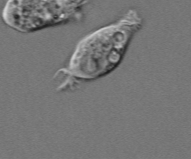
\includegraphics[width=0.4\paperwidth]{cell.png}}
    \caption{Original Image.}
\end{figure}

Το εργαστήριο έχει ως σκοπό την εξοικείωση μας με τις έννοιες μορφολογικής επεξεργασίας εικόνας. Πιο συγκεκριμένα καλούμαστε
να αναγνωρίσουμε το περίγραμμα του παραπάνω κυττάρου με ακρίβεια. Αυτό θα το επιχειρήσουμε χρησιμοποιώντας την μέθοδο Otsu
καθώς και μορφολογικές τεχνικές όπως erode και dilate συνδιασμένες με ποικίλα structuring elements.

\section{Ανάλυση}

\subsection{Max - Min}
Πριν εφαρμόσουμε την μέθοδο του Otsu, έπρεπε να γίνει ένα edge detection στην φωτογραφία, καθώς αν δεν το κάναμε θα είχαμε
μόνο την φωτεινή μεριά του περιγράμματος. Μετά απο αρκετό πειραματισμό, καθώς δεν θελαμε να χρησιμοποιήσουμε την μέθοδο
\textit{edge()} του matlab, καταλήξαμε να χρησιμοποιούμε τεχνικές από το προηγούμενο εργαστήριο. Πιο συγκεκριμένα, εξάγαμε
τις ελάχιστες τιμές της εικόνας και τις αφαιρέσαμε από τις μέγιστες χρησιμοποιώντας έναν 5x5 kernel. Αυτό μας έδωσε ένα
ομοιόμορφο περίγραμμα από το οποίο και μείναμε ικανοποιημένοι. Κάτι αντίστοιχο θα μπορούσε ίσως να επιτευχθεί χρησιμοποιόντας
και την αντίστοιχη διαφορά από morphological opening και closing. Στο παρακάτω figure, μπορεί κανείς να δει τα αποτελέσματά μας.

\begin{figure}[h]
    \centering
    \makebox[\textwidth]{\includegraphics[width=\paperwidth]{1.jpg}}
    \caption{Our Edge Detection Approach.}
\end{figure}
\clearpage

\subsection{EdgeDetection and Otsu}
Στην συνέχεια, χρησιμοποιήσαμε πάνω στο παραπάνω αποτέλεσμα την υλοποίησή μας από το προηγούμενο εργαστήριο για
edge-detection χρησιμοποιώντας το φίλτρο F=[-1 0 1] και την συνάρτηση μας \textit{convolution\_bonus()}. Τέλος,
χρησιμοποιήσαμε στο αποτέλεσμα αυτό τις συναρτήσεις \textit{graythresh()} και \textit{im2bw()} προκειμένου
να εξάγουμε ένα κατώφλι και να κάνουμε την εικόνα binary.

\begin{figure}[h]
    \centering
    \makebox[\textwidth]{\includegraphics[width=\paperwidth]{2.jpg}}
    \caption{Otsu Method Result.}
\end{figure}
\clearpage

\subsection{Contour Connection}
Λόγω τις προηγούμενης επεξεργασίας, έχουμε ήδη ένα αρκετά καλό αποτέλεσμα και θα μπορούσαμε να συνεχίσουμε έτσι στο επόμενο
βήμα. Παρ` όλ' αυτά, επιλέξαμε να χρησιμοποιήσουμε ένα structuring element δίσκου ακτίνας 12 ως όρισμα στη συνάρτηση
\textit{imtophat()} και πήραμε ένα μικρό, αλλά αποτελεσματικό smoothing στο περίγραμμα. έπειτα χρησιμοποιήσαμε την
\textit{imfill()} με το όρισμα `holes' και έτσι είχαμε πλέον αναγνωρήσει όλη την περιοχή του κυττάρου. Το αποτέλεσμα
φαίνεται παρακάτω.

\begin{figure}[h]
    \centering
    \makebox[\textwidth]{\includegraphics[width=\paperwidth]{3.jpg}}
    \caption{Dilate and fill.}
\end{figure}
\clearpage

\subsection{Erode}
Μετα, έπρεπε να μικρύνουμε ελαφώς το περίγραμμα καθώς λόγω της μεθοδολογίας μας ήταν ελαφρώς διογκωμένο.
Επιλέξαμε να χρησιμοποιήσουμε δύο φορές την \textit{imerode('diamond',1)}, χρησιμοποιήθηκε το συγκεκριμένο
structuring element επειδή θέλαμε να εφαρμοστεί κυρίως στις έντονες καμπύλες του περιγράμματος.

Και τέλος αφαιρέσαμε το κύταρρο που δεν θέλαμε να αναγνωρίσουμε μέσω της συνάρτησης \textit{imerode}.

Παρακάτω φαίνονται τα τελικά μας αποτελέσματα.

\begin{figure}[h]
    \centering
    \makebox[\textwidth]{\includegraphics[width=\paperwidth]{4.jpg}}
    \caption{Eroded, cleared-boarder and results.}
\end{figure}
\clearpage

\clearpage
\section{Κώδικας}
\matlabscript {main_5}{Η main.}
\matlabscript {convolution_bonus}{Η συνάρτηση edge-detection.}
\matlabscript {Compute_Min}{Η συνάρτηση Compute Min.}
\matlabscript {Compute_Max}{Η συνάρτηση Compute Max.}

\end{document}
